\section{Mechanisms}\label{mechanisms}

\subsection{Checks before spending}\label{checks-before-spending}

Deterministic checks run before every stage that costs money, because a fault is free to fix in the plan and costly once built. They test real geometry: light leaks, blocked openings, doors, open, thin or leaning models, and colours off the palette. The close-ups' shape check measures framing and outline, and an open vision-language model, Qwen3.8-27B \citep{qwen38}, compares each picture with its crop; it leans towards failing, because a wrong picture that passes costs a bad 3D model (Appendix C). Loose objects are dropped in a physics simulation, and one that would move further than a small limit fails the resting check, because a large move is a fault of the layout. A failed check sends the work back one stage (Appendix B).

Coding agents judging their own scenes agree with a measured score on geometry only 45.8 percent of the time \citep{li2026lego}, so a completion gate passes a place only when every inventory row has its object or a written reason, nothing visible stands in for a made piece, no resting fault is left, every model the creator picked is still the one shown, and every check ran on the stage as it is now; unknown blocks like fail, and a hook refuses to end an agent's session that claims a place is done while its gate does not pass.

\subsection{The parts check}\label{the-parts-check}

\begin{figure}
\centering
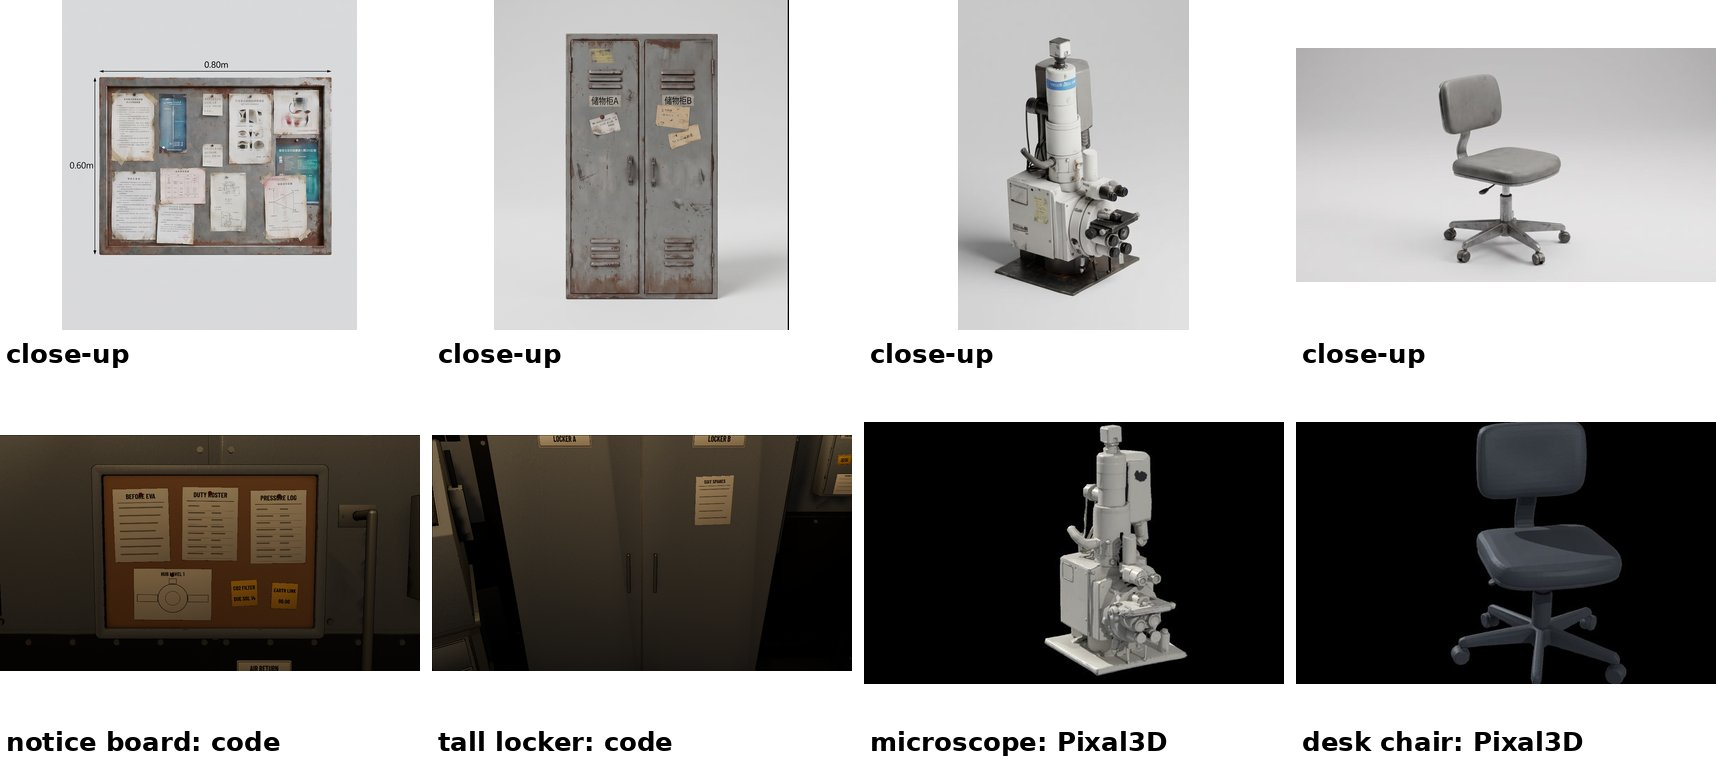
\includegraphics[width=0.7\linewidth,height=\textheight,keepaspectratio,alt={The parts check: four close-ups (top) and the objects as built (bottom). The notice board and locker are built in code, whose builds show every part; the microscope and chair are generated with Pixal3D.}]{figures/fig-parts-check.jpg}
\caption{The parts check: four close-ups (top) and the objects as built (bottom). The notice board and locker are built in code, whose builds show every part; the microscope and chair are generated with Pixal3D.}
\end{figure}

Picture-to-3D models build chunky solids well, but flat panels, thin beams and openings badly, while code builders are exact but show only the parts the coding agent wrote. For each kind of object, the parts check renders a code build from the front: if every part of the close-up is visible in it, the kind is built in code, and otherwise it is generated and made solid (Figure 3).

\begin{center}\fbox{\begin{minipage}{0.94\linewidth}\setlength{\parskip}{4pt}\small

\textbf{Gap: the parts check's order.} A queued change makes the parts check try generation first; this section is rewritten when it lands.

\end{minipage}}\end{center}

\subsection{Shape and surface apart}\label{shape-and-surface-apart}

\begin{figure}
\centering
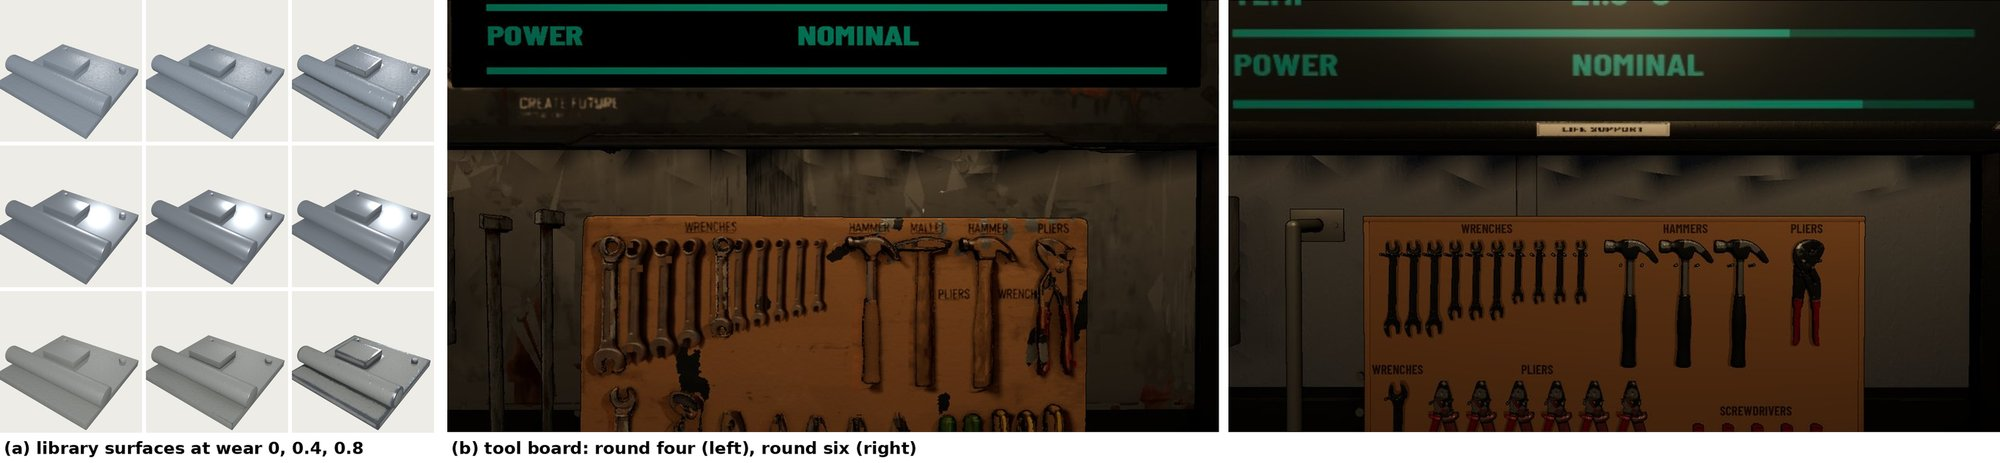
\includegraphics[width=0.7\linewidth,height=\textheight,keepaspectratio,alt={(a) Three library surfaces at wear 0, 0.4 and 0.8. (b) The hub's tool board with each piece's own picture colours (left) and with library surfaces, one model per tool (right).}]{figures/fig-surfaces.jpg}
\caption{(a) Three library surfaces at wear 0, 0.4 and 0.8. (b) The hub's tool board with each piece's own picture colours (left) and with library surfaces, one model per tool (right).}
\end{figure}

Every part of every object takes one surface from a shared library of rule-based surfaces, written as ProcFunc functions \citep{raistrick2026procfunc} on Infinigen's shaders \citep{raistrick2023infinigen}, coloured from the place's palette and worn only where wear has a cause, such as edges (Figure 4a, Appendix D). PartCrafter \citep{lin2025partcrafter} splits a generated model into parts, and an open vision-language model, shown each part outlined on the close-up, names its library surface; the picture's colours are not kept. When each piece kept them, every piece brought its own rust and stains (Figure 4b); with shape and surface apart, the hub became consistent and the creator accepted it (Appendix A).

\begin{center}\fbox{\begin{minipage}{0.94\linewidth}\setlength{\parskip}{4pt}\small

\textbf{Gap: painting beyond the hub.} On the rest of world 1 the painting is not yet consistent (Limitations). The surface stage's new method, to be measured there, is the finish-map route: Gemini 3.1 Pro \citep{gemini31pro} lists a model's finishes on its close-up and names a library surface for each, Nano Banana Pro draws the close-up again with one flat colour per finish, and SegviGen \citep{li2026segvigen} lays that map onto the shape.

\end{minipage}}\end{center}

\subsection{Review tools}\label{review-tools}

A review page, built only from the files the stages wrote, shows each stage's output, before-and-after shots from the same cameras, every check's result, and the stage rendered by Blender along a walk through it. An optional world step can turn the concept into a walkable room to show what the concept does not; nothing it produces is shipped.
